\documentclass{beamer}

\usetheme{Copenhagen}

\usepackage[utf8]{inputenc}
\usepackage[ddmmyyyy]{datetime}

% math
\usepackage{amsfonts}
\usepackage{amsmath}
% images
\usepackage{graphicx}
\graphicspath{ {../report/images/} }

\title{Warehouse allocation}
\author{Jakub Rada}
\date{3.1.2022}

\begin{document}

\begin{frame}
    \titlepage
\end{frame}

\begin{frame}
    \frametitle{Problem description}

    \begin{itemize}
        \item $N$ warehouses, $M$ customers
        \item set-up price $s_w$, capacity $cap_w$ $\qquad \forall w = 1, \dots, N$
        \item demand $d_c$ $\qquad \forall c = 1, \dots, M$
        \item delivery cost $t_{cw}$ $\qquad \forall c = 1, \dots, M \quad w = 1, \dots, N$
    \end{itemize}

    \begin{equation*}
        \begin{array}{ll @{} ll}
            \text{minimize}   & f = \displaystyle\sum_{w = 1}^{N}(I(|a_w| > 0) \cdot s_w + \sum_{c \in a_w} t_{cw}) & \\
            \text{subject to} & \displaystyle\sum_{c \in a_w} d_c \leq cap_w & \forall w = 1, \dots, N \\
                              & \displaystyle\sum_{w = 1}^{N} I(c \in a_w) = 1 & \forall c = 1, \dots, M \\
        \end{array}
    \end{equation*}
\end{frame}

\begin{frame}
    \frametitle{Representation and fitness function}
    \begin{block}{Candidate}
        \begin{center}
            \begin{tabular}{| c | c | c | c | c |}
                \multicolumn{1}{c}{$1$} & \multicolumn{1}{c}{$2$} & \multicolumn{1}{c}{$\cdots$} & \multicolumn{1}{c}{$M - 1$} & \multicolumn{1}{c}{$M$} \\
                \hline
                $w_1$ & $w_2$ & $\cdots$ & $w_{M-1}$ & $w_M$ \\
                \hline
            \end{tabular}
        \end{center}
    \end{block}
    \begin{block}{Fitness function}
        \begin{itemize}
            \item fitness $f$
            \item constraint violations $g = \displaystyle\sum_{w = 1}^{N}\max(0, \sum_{c \in a_w} d_c - cap_w)$
        \end{itemize}
        \begin{enumerate}
            \item $h = f + a \cdot g \qquad a \in \mathbb{R}$
            \item $c_1$ is better than $c_2$ \textit{if} $g(c_1) < g(c_2) \text{ or } (g(c_1) = g(c_2) \text{ and } f(c_1) < f(c_2))$
        \end{enumerate}
    \end{block}
\end{frame}

\begin{frame}
    \frametitle{Local search}
    \begin{itemize}
        \item standard local search with first-improving strategy
    \end{itemize}
    \begin{block}{Candidate is invalid}
        Find assignment of warehouse with exceeded capacity and change it randomly. If it improved, keep it and find another.
    \end{block}
    \begin{block}{Candidate is valid}
        Randomly change one assignment.
    \end{block}
\end{frame}

\begin{frame}
    \frametitle{EA}
    \begin{itemize}
        \item Population size: $50$
        \item Selection: $5$ parents using tournament selection
        \item Crossover: breed all pairs of parents with single point crossover
        \item Mutation: randomly change one assignment with probability $0.5$ or randomly shuffle assignments with probability $0.3$
    \end{itemize}
\end{frame}

\begin{frame}
    \frametitle{Memetic algorithm}
    \begin{itemize}
        \item Population size: $20$
        \item Selection: $5$ parents using tournament selection
        \item Crossover: breed all pairs of parents with uniform crossover
        \item Mutation: randomly change one assignment with probability $0.2$ or randomly shuffle assignments with probability $0.6$
    \end{itemize}
    \begin{block}{Local search}
        After breeding phase, run 100 iterations of local search on each offspring with probability $0.3$.
        In each iteration a mutation operator is selected with probability $0.5$.

        Mutation operators:
        \begin{itemize}
            \item randomly change $n$ assignments
            \item find the most expensive assignment and replace it with cheapest
        \end{itemize}
    \end{block}
\end{frame}

\begin{frame}
    \frametitle{Experiments}
    \begin{itemize}
        \item 8 instances

    \begin{tabular}{ c | c | c | c }
        & customers & warehouses & optimal solution \\
        \hline
        wl\_16\_1   & 50 & 16 & 976738.625 \\
        wl\_25\_2   & 50 & 25 & 796648.438 \\
        wl\_50\_1   & 50 & 50 & 793439.562 \\
        wl\_100\_4  & 1000 & 100 & 17765201.949 \\
        wl\_200\_1  & 200 & 200 & 2686.479 \\
        wl\_500\_1  & 500 & 500 & 2608.148 \\
        wl\_1000\_1 & 1000 & 1000 & 5283.757 \\
        wl\_2000\_1 & 2000 & 2000 & 10069.803 \\
    \end{tabular}
        \item fitness function evaluations range from $1000$ to $5000000$
        \item each solved 11 times
    \end{itemize}
\end{frame}

\begin{frame}
    \frametitle{Experiments}
    \begin{itemize}
        \item valid solution found after 1000 evaluations every time
        \item memetic algorithm is significantly better on large instances, on smaller ones is slightly behind ls and ea
        \item ea is by far the slowest, ls fastest
    \end{itemize}
\end{frame}

\begin{frame}
    \frametitle{wl\_16\_1}
    \begin{minipage}{0.5\textwidth}
        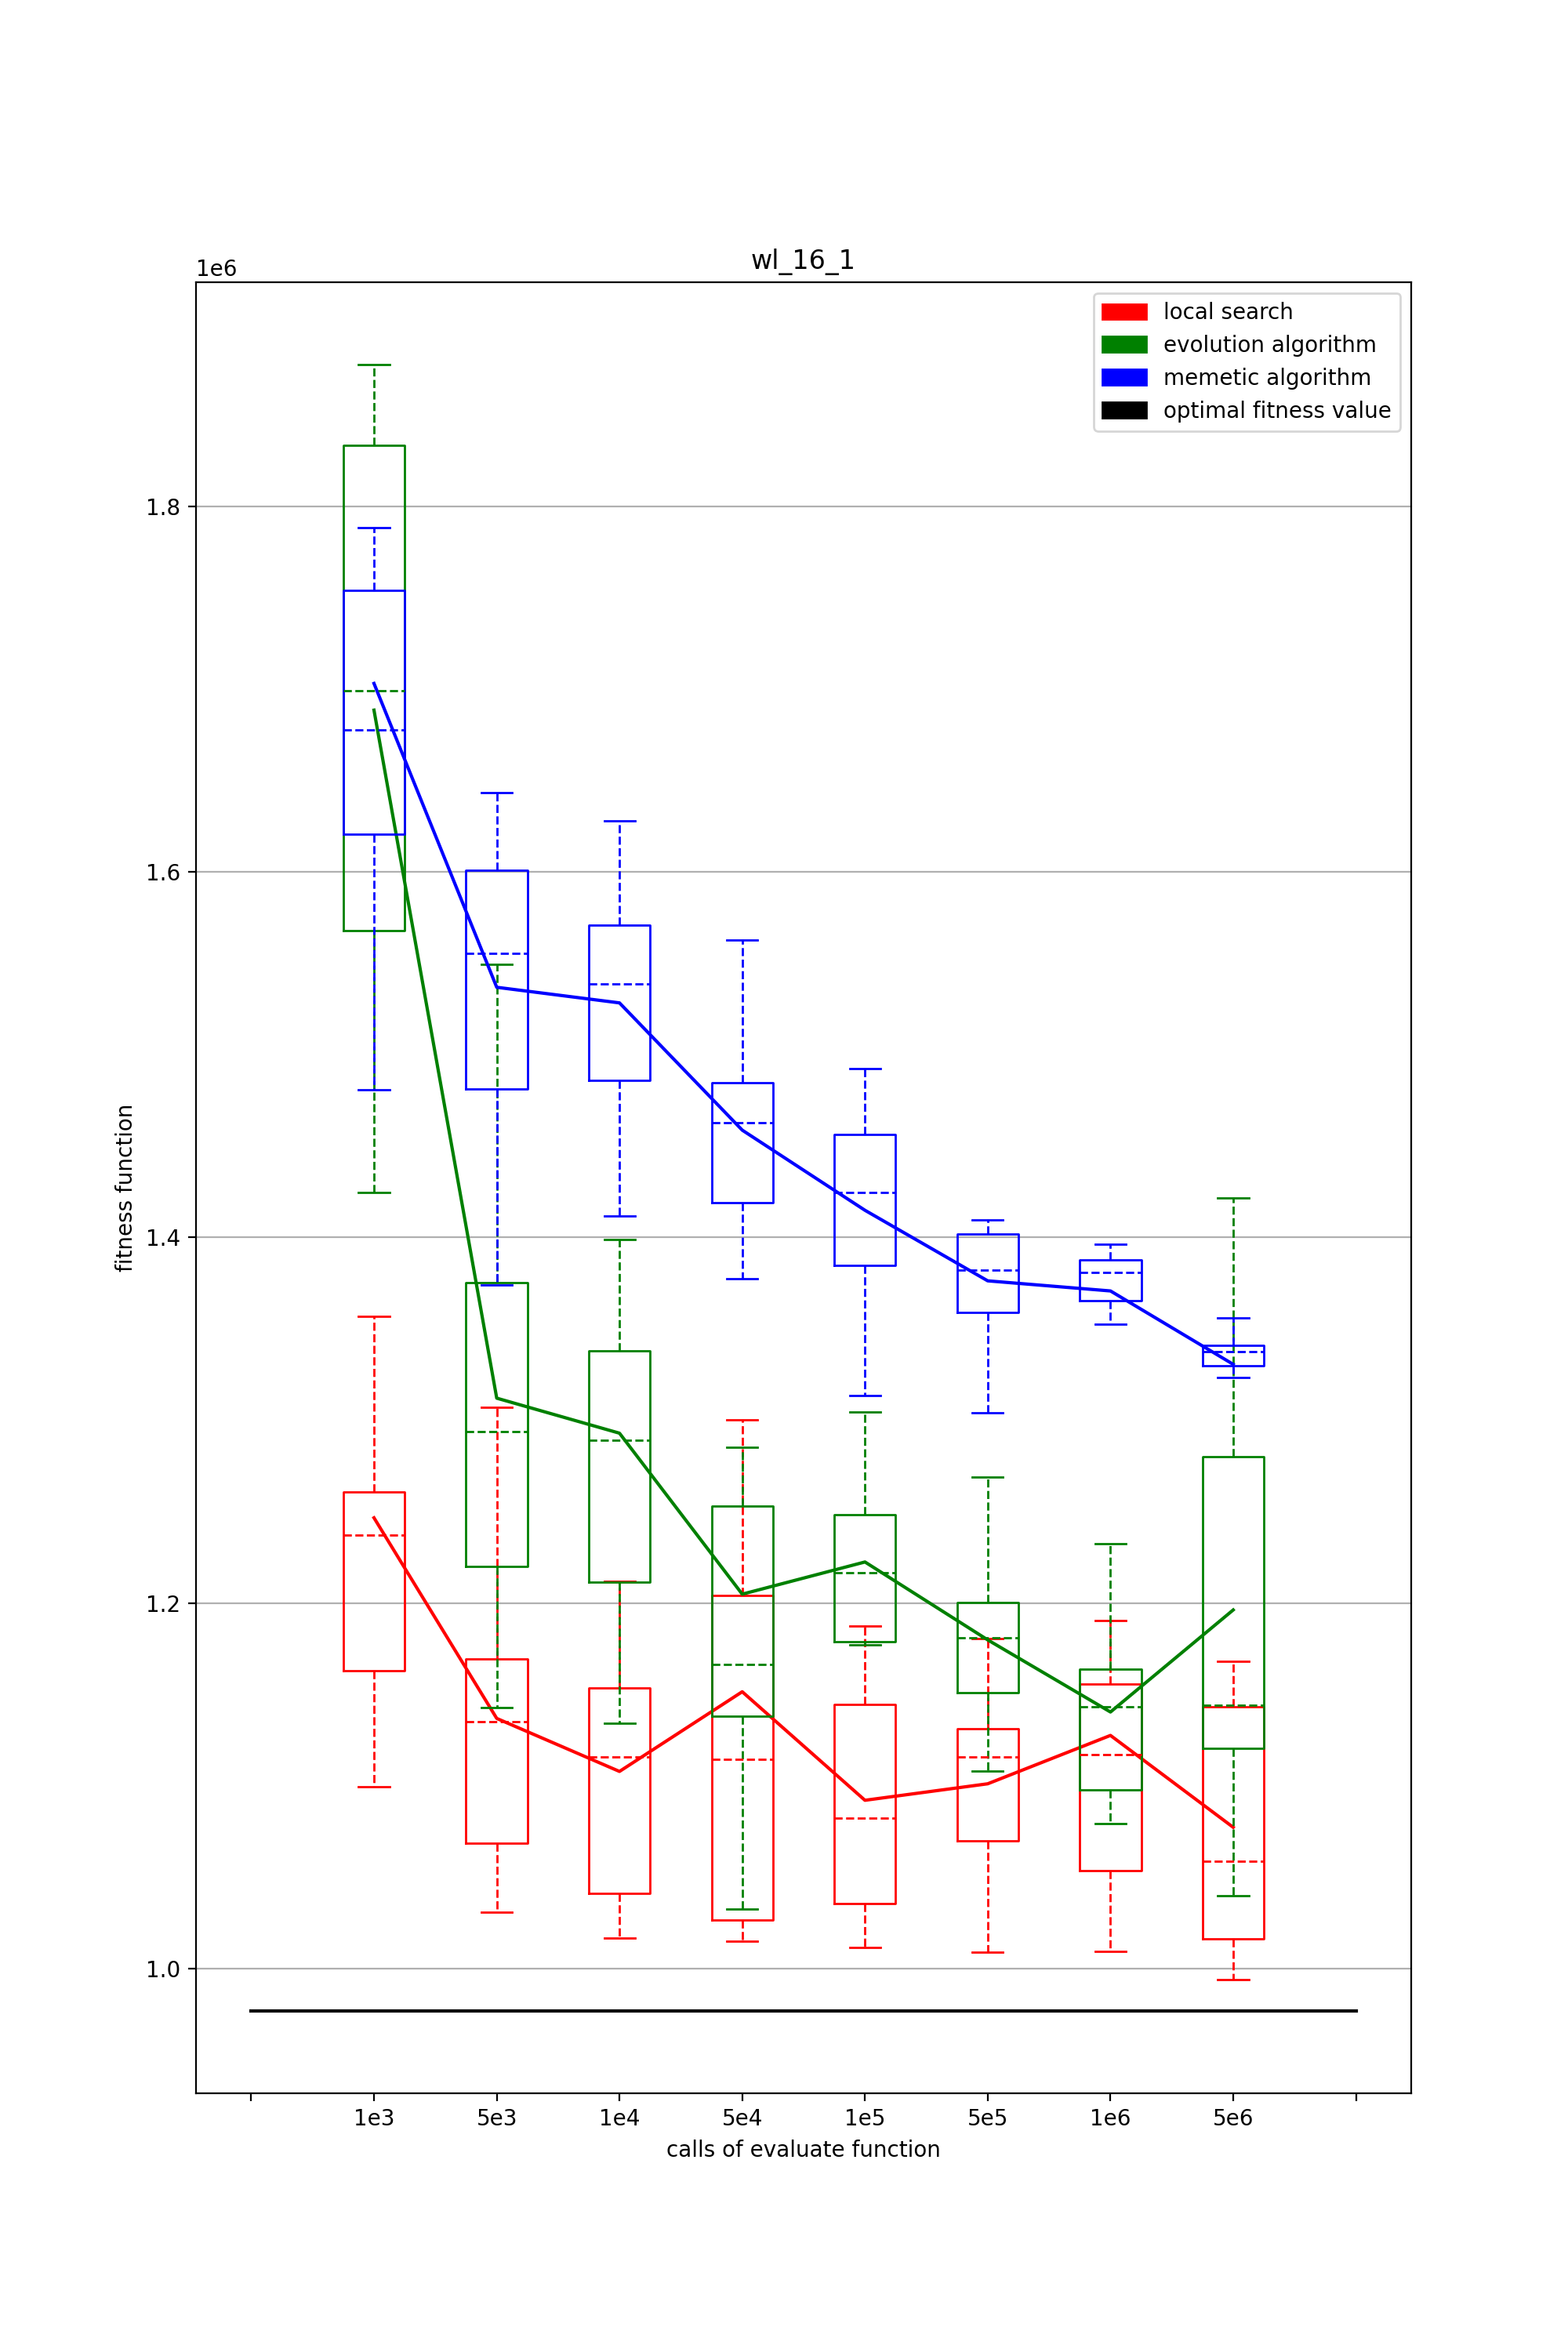
\includegraphics[width=\textwidth]{wl_16_1.png}
    \end{minipage}
    \begin{minipage}{0.4\textwidth}
        \begin{tabular}{ c | c | c }
            M & N & optimum \\
            \hline
            50 & 16 & 976738.625 \\
        \end{tabular}
        \begin{table}
            \centering
            \begin{tabular}{ c | c | r }
                algorithm & value & ratio \\
                \hline
                ls & 993907.0 & 1.02 \\
                ea & 997198.0 & 1.02 \\
                memetic & 1266930.0 & 1.3 \\
            \end{tabular}
            \caption{Best found solutions}
        \end{table}
    \end{minipage}
\end{frame}

\begin{frame}
    \frametitle{wl\_100\_4}
    \begin{minipage}{0.5\textwidth}
        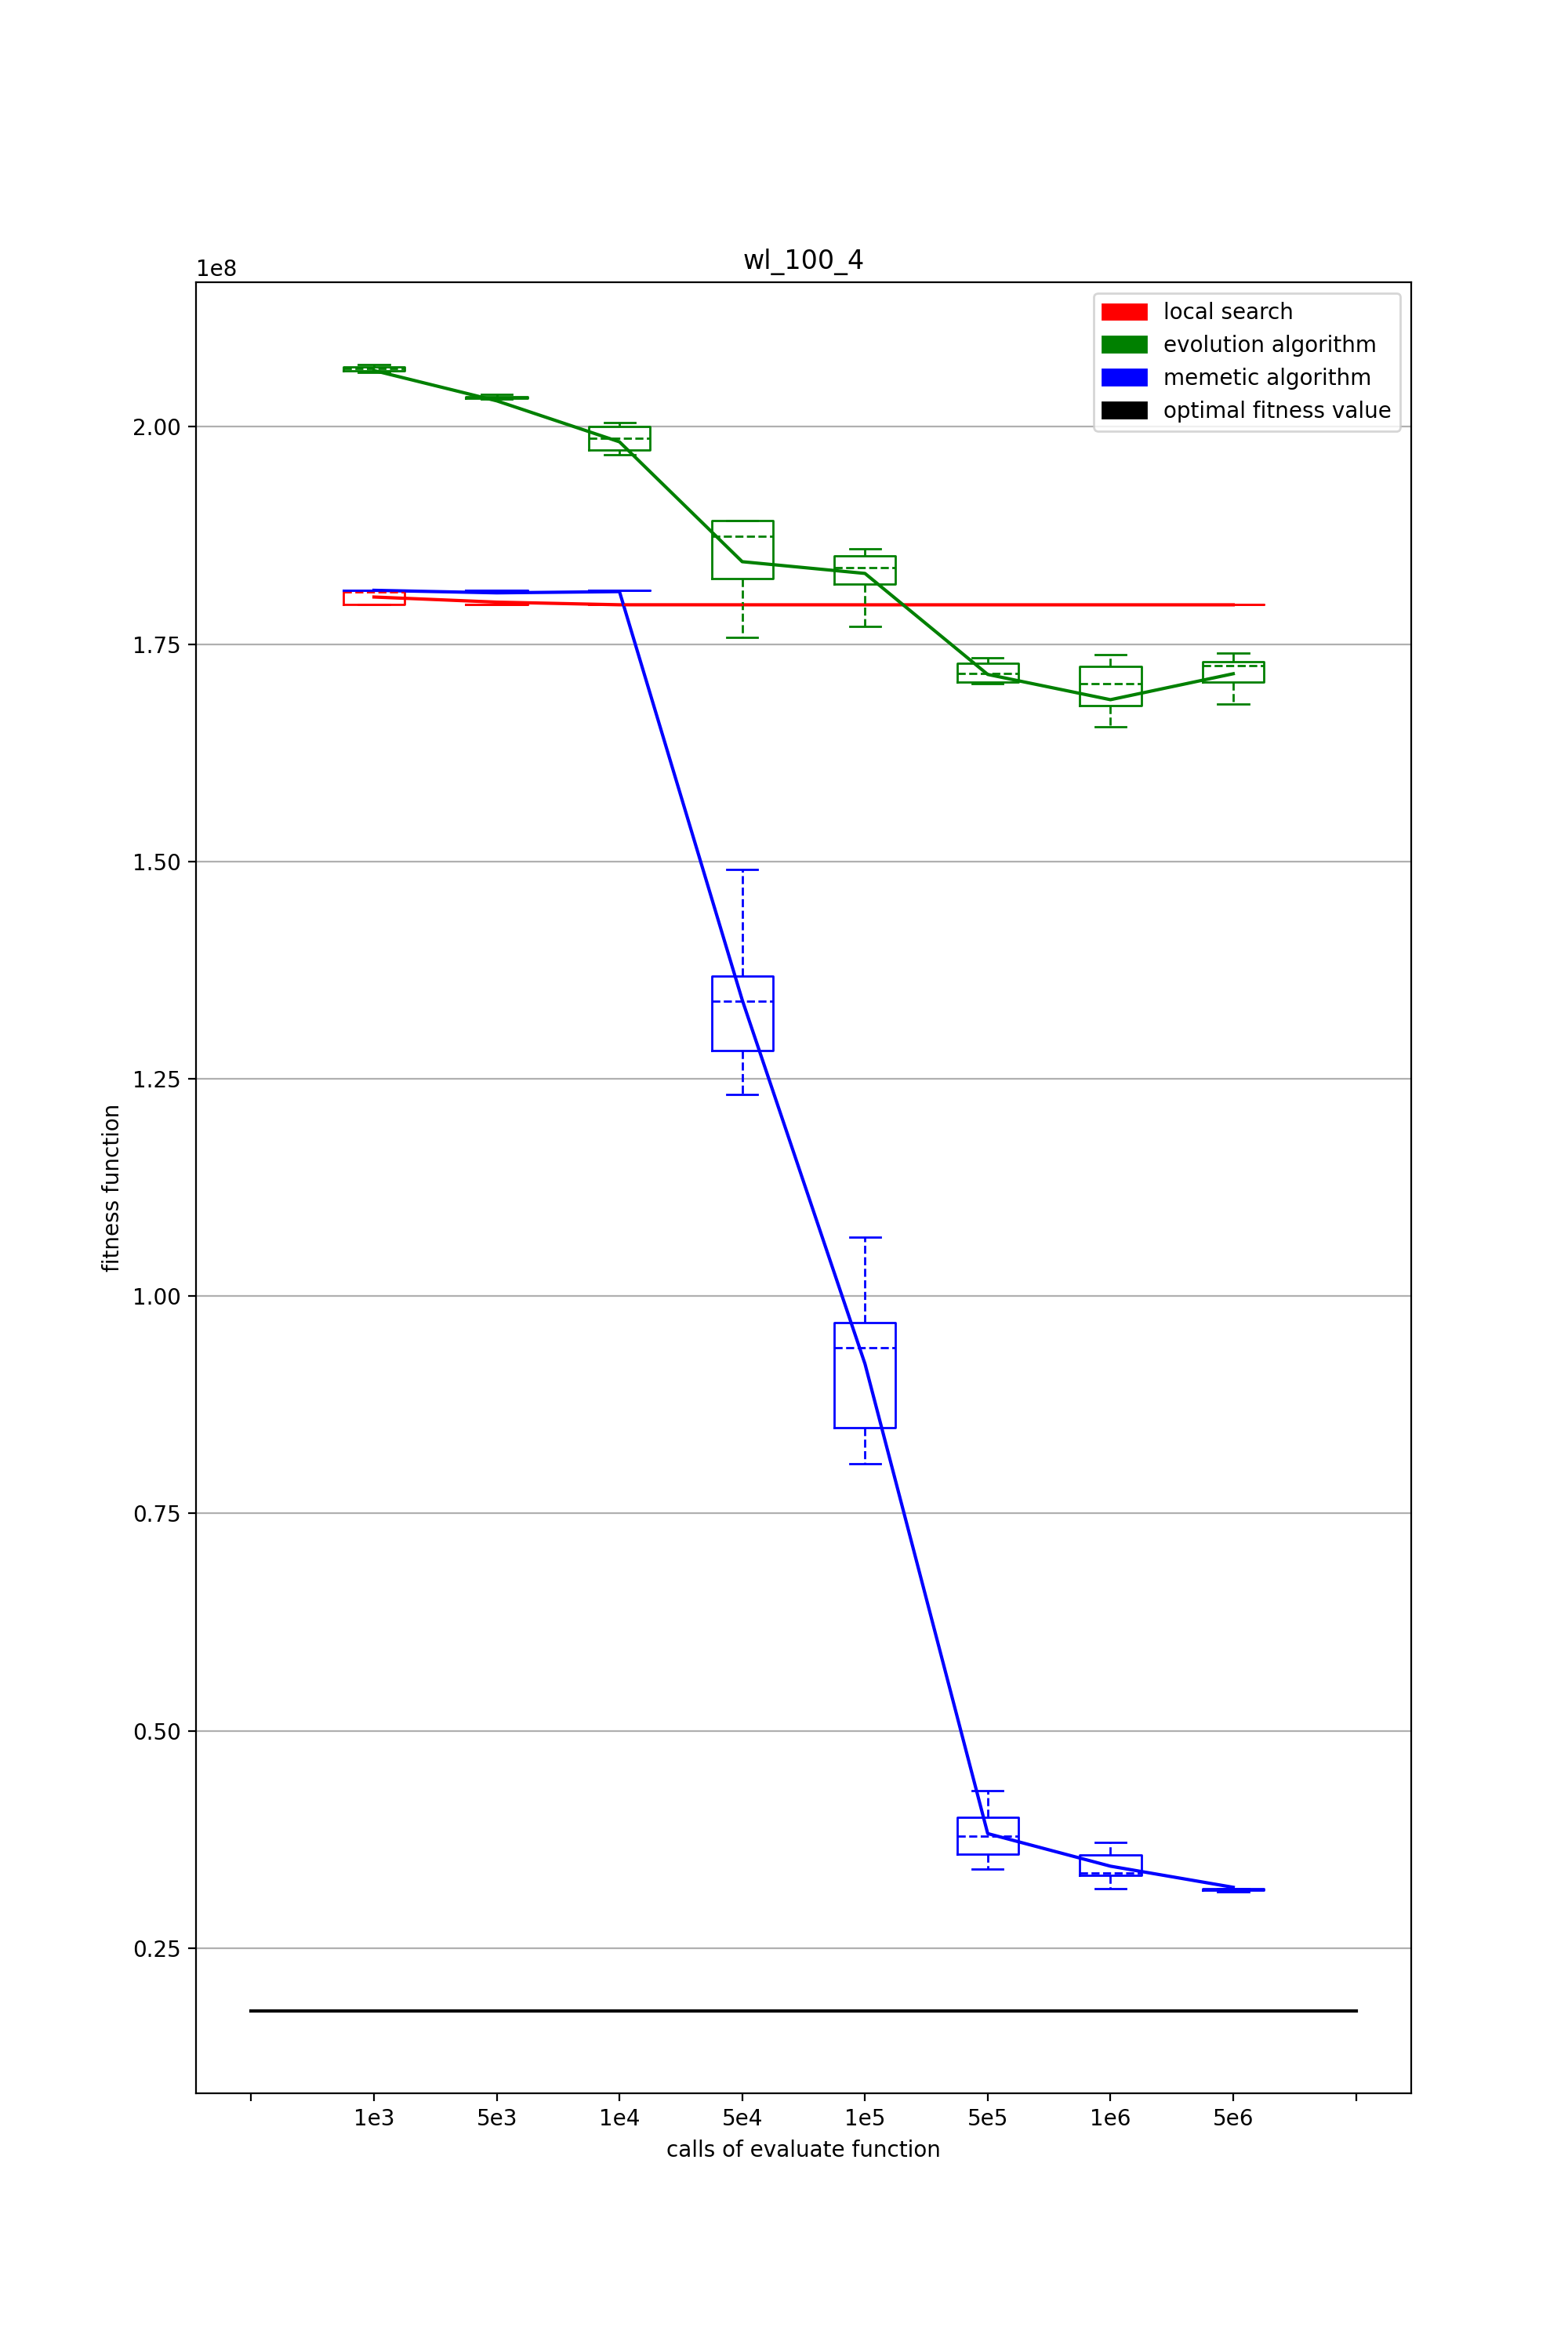
\includegraphics[width=\textwidth]{wl_100_4.png}
    \end{minipage}
    \begin{minipage}{0.4\textwidth}
        \begin{tabular}{ c | c | c }
            M & N & optimum \\
            \hline
            1000 & 100 & 17765201.949 \\
        \end{tabular}
        \begin{table}
            \centering
            \begin{tabular}{ c | c | r }
                algorithm & value & ratio \\
                \hline
                ls & 1.80e8 & 10.11\\
                ea & 1.65e8 & 9.31\\
                memetic & 3.14e7 & 1.77\\
            \end{tabular}
            \caption{Best found solutions}
        \end{table}
    \end{minipage}
\end{frame}

\begin{frame}
    \frametitle{wl\_2000\_1}
    \begin{minipage}{0.5\textwidth}
        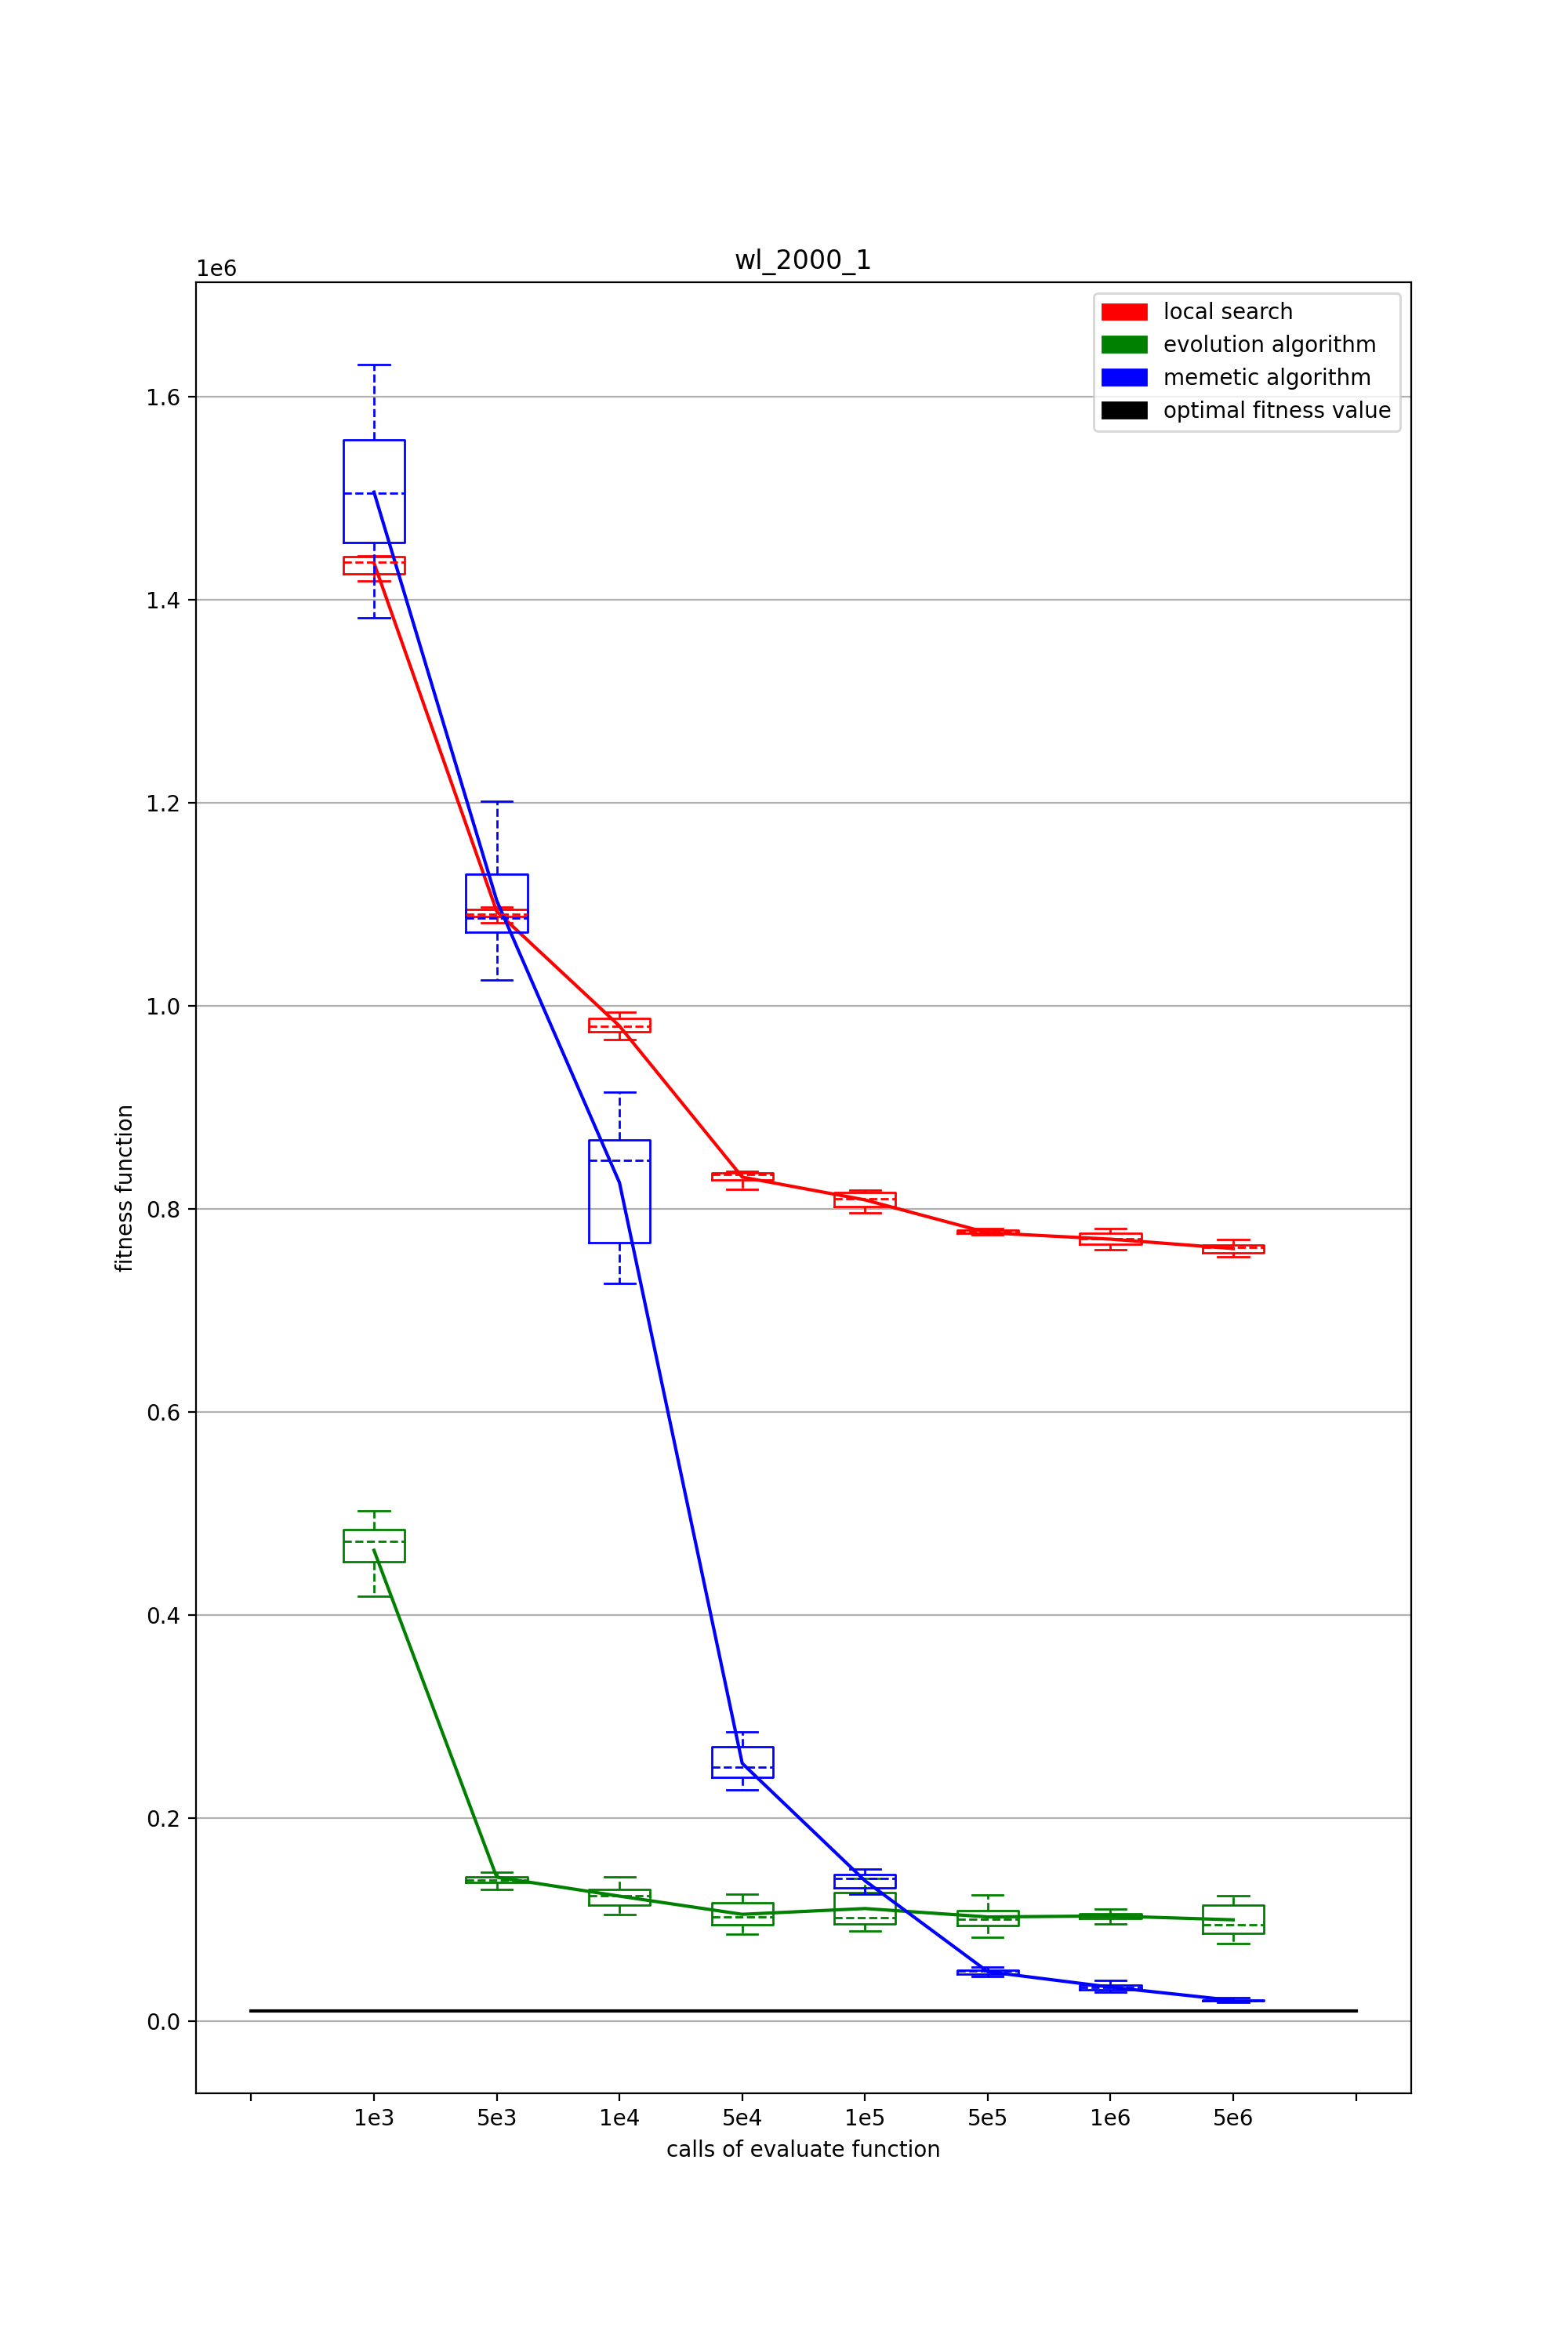
\includegraphics[width=\textwidth]{wl_2000_1.png}
    \end{minipage}
    \begin{minipage}{0.4\textwidth}
        \begin{tabular}{ c | c | c }
            M & N & optimum \\
            \hline
            2000 & 2000 & 10069.803 \\
        \end{tabular}
        \begin{table}
            \centering
            \begin{tabular}{ c | c | r }
                algorithm & value & ratio \\
                \hline
                ls & 7.53e5 & 74.78 \\
                ea & 7.65e4 & 7.56 \\
                memetic & 1.85e4 & 1.84 \\
            \end{tabular}
            \caption{Best found solutions}
        \end{table}
    \end{minipage}
\end{frame}

\end{document}

